% Options for packages loaded elsewhere
\PassOptionsToPackage{unicode}{hyperref}
\PassOptionsToPackage{hyphens}{url}
%
\documentclass[
]{article}
\usepackage{amsmath,amssymb}
\usepackage{lmodern}
\usepackage{iftex}
\ifPDFTeX
  \usepackage[T1]{fontenc}
  \usepackage[utf8]{inputenc}
  \usepackage{textcomp} % provide euro and other symbols
\else % if luatex or xetex
  \usepackage{unicode-math}
  \defaultfontfeatures{Scale=MatchLowercase}
  \defaultfontfeatures[\rmfamily]{Ligatures=TeX,Scale=1}
\fi
% Use upquote if available, for straight quotes in verbatim environments
\IfFileExists{upquote.sty}{\usepackage{upquote}}{}
\IfFileExists{microtype.sty}{% use microtype if available
  \usepackage[]{microtype}
  \UseMicrotypeSet[protrusion]{basicmath} % disable protrusion for tt fonts
}{}
\makeatletter
\@ifundefined{KOMAClassName}{% if non-KOMA class
  \IfFileExists{parskip.sty}{%
    \usepackage{parskip}
  }{% else
    \setlength{\parindent}{0pt}
    \setlength{\parskip}{6pt plus 2pt minus 1pt}}
}{% if KOMA class
  \KOMAoptions{parskip=half}}
\makeatother
\usepackage{xcolor}
\IfFileExists{xurl.sty}{\usepackage{xurl}}{} % add URL line breaks if available
\IfFileExists{bookmark.sty}{\usepackage{bookmark}}{\usepackage{hyperref}}
\hypersetup{
  pdftitle={Do You Garden?},
  pdfauthor={Olivia Lucca Fraser},
  hidelinks,
  pdfcreator={LaTeX via pandoc}}
\urlstyle{same} % disable monospaced font for URLs
\usepackage{graphicx}
\makeatletter
\def\maxwidth{\ifdim\Gin@nat@width>\linewidth\linewidth\else\Gin@nat@width\fi}
\def\maxheight{\ifdim\Gin@nat@height>\textheight\textheight\else\Gin@nat@height\fi}
\makeatother
% Scale images if necessary, so that they will not overflow the page
% margins by default, and it is still possible to overwrite the defaults
% using explicit options in \includegraphics[width, height, ...]{}
\setkeys{Gin}{width=\maxwidth,height=\maxheight,keepaspectratio}
% Set default figure placement to htbp
\makeatletter
\def\fps@figure{htbp}
\makeatother
\setlength{\emergencystretch}{3em} % prevent overfull lines
\providecommand{\tightlist}{%
  \setlength{\itemsep}{0pt}\setlength{\parskip}{0pt}}
\setcounter{secnumdepth}{-\maxdimen} % remove section numbering
\ifLuaTeX
  \usepackage{selnolig}  % disable illegal ligatures
\fi

\title{Do You Garden?}
\author{Olivia Lucca Fraser}
\date{2022-04-23}

\begin{document}
\maketitle
\begin{abstract}
Moving to the country, going to eat a lot of peaches.
\end{abstract}

\hypertarget{do-you-garden}{%
\section{Do You Garden?}\label{do-you-garden}}

\textbf{As Ashley massaged} the loose skin free from the flesh of a
boiled peach, the last one of one of the day's last batches, each batch
a batch of a dozen, at least, and then braced the paring knife's blunt
edge against the blistered pad of his thumb, numbed from being plunged
into the mostly molten ice to fish out one peach after another, his
thoughts would gather in the familiar hollow the familiar work hollowed
out. These concerned his wife.

When knife bit into the peach pit, he rolled it full circle and thought
of Sheila, his wife, and with a twist split open the peach. He scooped
up the slippery halves of the peach and with a thought of his wife they
lept from his hands to the jar like pair of koi. And with thoughts of
her came thoughts of the fire and the rest revolved around these. Now
and then these thoughts were eclipsed by thoughts of the nurse, Javier,
as when he gathered the pits in an ice-cream bucket that the sun had
bleached a dull green.

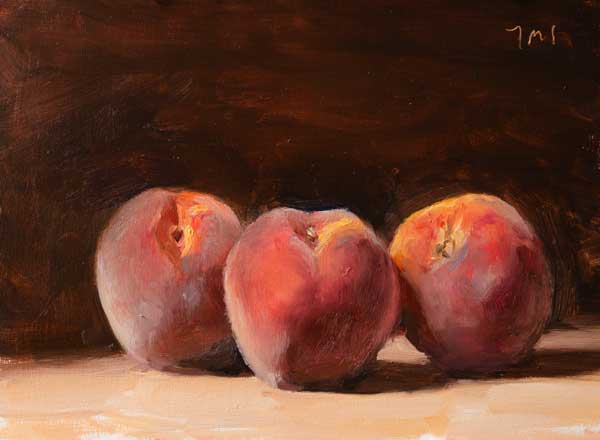
\includegraphics{../img/peaches.jpg}

His flipflops made a puckering, sucking sound as he moved to stir the
syrup and lower the flame a notch, and set the sprawling glass honeycomb
of mason jars tinkling. The afternoon light on the pine-pannelled walls,
beaded with varnish that never quite dried, and gave an amber cast to
the kitchen, into which the smell of peaches had steadily been luring
wasps. On three separate occasions, Ashley had had to dump an entire jar
of peaches into a dull yellow colander and hose them off in the sink,
pressing his still-unblistered thumb hard up against the faucet so that
the water would spray with sufficient force to dislodge the wasp from
her dinner and push her twitching, brittle body through the slits in the
pasta strainer. Each time it made him shudder. After the third occasion
he had to pause to gather his nerves again and look out over the
orchard, from the window over the sink. The afternoon was overcast, and
the light had the sort of grayness to it that made everything out there
gray. An engineless glider, so close to the cloud cover's colour that
only movement gave it away, turned in broad and patient arcs. Something
twitched up close at the edge of the frame. Something with brassy legs
and antennae and a lithe black body that glistened and flexed a wisplike
ovipositor. It coiled and uncoiled and coiled again with horribly
intimate urgency. Ashley heard himself shout ``stumpfucker!'' and
scrambled about for something. Everything around him a weapon. He
grabbed an open bottle of Joy and smashed the bug with the butt of it,
before it could climb through the hole in the screen. Yellow ropes of
soap shot back in his direction. He smashed it again and again and when
he separated the wasp from its abdomen and it still wouldn't stopped
twitching he dropped the bottle and frantically yanked the empty tin can
of pineapple juice that had been propping up the sash. The window
slammed shut so hard and so fast that for an instant he thought it would
crack.

The peaches in the colander were covered in soap. With them were three
or four pieces from the modest collection of beach glass he had arranged
in a row on the window sill, the summer they'd first moved into the
cabin.

``Ashley?'' said Javier's baritone voice, and Ashley looked up to see
him behind him. He'd silently entered the kitchen, wearing his indoor
sneakers and egg-white scrubs. ``Are you hurt?''

``No, no, sorry, no, it was just a stu -- just a wasp, a big wasp. In
the, uh --''

``Are you allergic?''

``No.~Sorry. No, I'm okay.''

``Here,'' he said, unzipping a burgandy fanny pack and rooting around
inside it, ``let me get you some lotion.''

``No, sorry, I'm, I'm okay, I didn't get stung. I'm okay. I got it.''

``I'd hate to see the other guy,'' said Javier, smiling.

``Oh, huh, yeah, yeah, I got him good,'' said Ashley. ``How's Sheila?''

``She's fine. She's a very intelligent woman, very wise,'' Javier nodded
dreamily and chuckled, ``clearly, you know this.''

``The, uh\ldots{}'' Ashley trailed off.

``No, of course, she's still on fire,'' said Javier, ``there's been no
change in the fire,'' which Ashley did not find surprising, of course,
but it would have felt strange not to ask. He breathed in, and smiled
again. ``Ashley, it smells divine in here. We both look forward to your
peaches, Ashley. We very much look forward to them.'' Javier turned to
exit the kitchen, paused, with his ear cocked lifted and rested his
foot, and then fished a wet-nap from his fannypack and wiped the sugar
from the soles of his tennis shoes, before returning to the master
bedroom.

It had been three full years since the fire began, which was, in itself,
unusual. But no more unusual than two, to be fair, or even, for all
that, a week. Whether or not it was normal for someone in that state to
have a stomach only for peaches, there was no way, really, to know this.
He once asked his nutritionist cousin about it, but she'd just said, ``I
really don't know what to tell you. It's just not something I've seen
before.'' ``In your practice, you mean?'' Ashley asked, deferentially.
``No, not really at all, no,'' said his cousin. And Yahoo wasn't any
help either. It was unclear what to expect with these things, and the
fire itself was unusual, for fire, in that it didn't seem to hurt her,
for one, or even, really, to \emph{burn} her -- it didn't cause any
tissue damage, at least according to Javier. Nor did it spread to
anything that Sheila had come in touch with. When she'd first caught
fire, at least after they'd come to grips with it, they had both been
extremely cautious not to burn down the house. For an entire week Sheila
lived in the bathtub, and Ashley would bring her meals but she'd leave
them untouched, until they eventually hit on the peaches. On the flames
the water had no effect whatsoever, besides noisily sputtering, which
soon became sufficiently irritating that Sheila drained the tub out and
sat on the dry enamel. When she noticed, quite by accident, that it
didn't burn the curtain, they gingerly began to experiment. But the fire
clung to Sheila, alone. Or to flesh, alone, perhaps. The possibility
that it could spread to another human body was too dangerous to properly
test.

The difficult thing was his asthma.

The fire had never produced any smoke, at least nothing that looked like
smoke. But in time Ashley sensed that something was up with the air in
Sheila's vicinity. He started to develop an allergy, which he initially
wrote off as hayfever, and probably nothing more, but it persisted well
into winter and on a late afternoon in the middle of February he started
to notice the threads. They hung in the air all around her, within a ten
foot radius, and had a way of sliding slowly about that distinguished
them somehow from dust motes. ``They had a purposeful way of moving,''
is how he might have once described these ephemeral glassy filaments,
which congregated around her and in whose presence he could now scarcely
breathe.

Unlike the fire, about whose existence and gravity no one was in doubt
(and though theories about it varied, these don't concern us here), the
filaments troubled Ashley alone. Not only were they \emph{quite}
difficult to see, and under most slants of light invisible, but his
allergy to them seemed quite particular, perhaps an effect of prolonged
exposure. Every doctor he consulted seemed skeptical that there was
anything in the air, there, at all, and he suspected the friends who had
nodded and said, ``yes, yes I see what you mean,'' had been aiming only
to humour him. Neither loratadine nor cetirizine hydrochloride provided
any relief at all. Fexofenadine made the symptoms worse and
diphenhydramine made him drowsy. Exposing himself to the filaments for
even just a few seconds could spark a fit of coughing that would deprive
him of sleep for the night. And when he spotted the tiny red specks on
his sleeve, after a night of tossing and turning and coughing on the
hide-a-bed in the living-room -- where he'd been sleeping since Sheila
had taken the bed after an uncomfortable week in the bathtub -- he
decided to hire a nurse.

They got along well with Javier, who was always conscientious and
courteous. He would even make a point to bring gifts for the couple on
the occasion of every solemnity, including many of which Ashley, who had
been raised Catholic, himself, had to confess he'd been ignorant. On the
Assumption of Mary he presented to Ashley a bottle of Lepanto brandy,
and to Sheila modest pearl earrings. On All Saints' Day, he gave Ashley
\emph{Resolí} and Sheila a tasteful pearl brooch. On the Solemnity of
Our Lord Jesus Christ, King of the Universe, Ashley received a green
liqueur in a bottle shaped like a sine wave labelled \emph{Hierbas de
Malloreca}, and Sheila received a pearl necklace. And so it went,
without fail, and each gift came without ceremony. At first Ashley tried
to demure, and beckoned Javier into the sun porch that day (on the first
of the Assumptions in question) while \emph{Rigoletto} played loud on
the radio, and mumbled something about how Sheila, these days, didn't
have much use for jewelry, and that the fire would probably damage them
anyway (he knew that it wouldn't, it clung to her jealously, and never
scorched anything she wore), and that they couldn't, in any case, accept
these gifts, it's enough that they pay him so little, but Javier only
shrugged and smiled and said it was no trouble at all. The pearls, the
jewelry, these were hobbies of his, and as for the liquors he'd
inherited them all when he'd inherited his father's house, and he,
himself, didn't drink.

Once the last of the batch of peaches was sliced up and jarred, Ashley
rinsed his hands and dried them on his khaki pants and slipped on a worn
pair of oven mitts. He carefully poured the syrup into a tin watering
can which he used to cover the fruit in each jar. Here and there a slice
of star anise would bob to the surface along with fragments of cinnamon
bark. After shooing the remaining wasps away, he placed the lids on the
jars and screwed on the rings. The big pot took ten at a time and he
wrapped each one in a thin cotton rag, strips of a ratty bedsheet, so as
to keep them from cracking when the water boiled and jostled them
against one another.

He fished a Red Bird match from a terra cotta pot on the dusty top of
the fridge and struck it against the side, and lit the large front
burner on the stove. The ignition switch had been broken for years,
despite his frequent vows to fix it. There was a time, in the first six
months of the fire, when he'd blame the stove for what happened, or at
least make an effort to do so, as a means of blaming himself. He'd
occasionally hear himself saying things like, ``I should never have let
you use that stove, not in your condition,'' but his voice would lilt at
``\emph{condition?}'' as if the apology were some sort of plea. It was
not for lack of feeling that the words lacked all conviction, being less
an empty vessel than a sieve. What \emph{condition}, after all, could he
have possibly meant? What dull-witted meaning did he expect would crawl
out of the woods and get tangled in that apologetic net? If his
intention was to draw out an avowal of guilt, or of the Hand of God at
work in this world, then he wriggled on that hook alone. What bothered
him most, as he heard himself speak, was the peculiar tone of his voice,
which he judged irredeemably mewling. He did make efforts to correct it,
and made a point to speak with his chest, like an actor. This, the
critic he once was would've written, ``had him delivering the lines
histrionically,'' or in a crueller temper, ``hamfistedly, failing to
stoke the slightest conviction and leaving the audience cold.''

His theatre critic days were in any case behind him, due to the
withering away of the fourth estate, in fact, only in part. His facility
with language had left him. The diaries he still kept and scribbled in
daily he could no longer bear to read. His worries clattered out of him
in clunky blocks of cliché. He was no longer at home with words.

The hallway pulsed with flickering light and the indecipherable end of a
bright conversation became for a moment unmuffled before giving way to
goodbyes as the door to the bedroom opened and shut and Javier returned
to the kitchen. ``You know, Ash,'' he said, while the canning pot boiled
and the mason jars mutely clattered about, ``she cares for you a great
deal. She has such appreciation for you. Do you know that?'' Ashley
nodded his head like a bobblehead doll and smiled at the warmth in his
voice. Javier removed his tennis shoes, placed them neatly by the door,
and pulled on his rubber boots. He lifted a heavy green raincoat from a
peg beside the door, and gripping the cuffs of his scrub sleeves so they
wouldn't ride up, he slowly put it on, without taking his eyes off
Ashley. ``I do hope you know that.'' He turned towards the door.

Fiddling with a peach stone he'd just finished scrubbing, Ashley said,
``oh, Javier, the, uh\ldots{} they're ready for you,'' in a voice that
felt flustered and stilted. ``The peach stones, I mean,'' he said,
nodding at the plastic ice cream bucket on the corner of the table.

``Ah, I almost forgot!'' Javier said, and moved to slide off his boots.

``It's fine,'' Ashley said, ``I have to mop anyway,'' at which Javier
shrugged, approached the bucket and checked its seal, pressing it tight
til it clicked on one side, and then gave it a shake and said, ``thank
you!''

``I've been\ldots{} I've been meaning to ask,'' said Ashley, ``what do
you, uh, I mean, do you garden?''

``Truly, Ash, thank you!'' said Javier, holding the bucket with a single
hand as if it were a large cup of coffee, ``I do appreciate this.''
Something outside the window caught Ashley's eye and he turned to see
what it was. ``And no, I don't garden,'' said Javier. ``But thank you.''
Javier lifted his backpack from the peg where his raincoat was hanging,
hefted it onto his shoulder, and then removed it again and unfastened
the flap. ``Ash, I almost forgot,'' he said, ``I have something for
you,'' and placed a tall bottle of \emph{Gusano Rojo} on the clear patch
of table where the pit bucket had stood.

``Thank you, you didn't have -- no, thank you,'' said Ashley. Javier
smiled broadly, and left.

Behind the muted clatter of jars it was quiet. Ashley cleared out the
sink and ran the tap, and waited for the water to get warm, restlessly
scanning the sky as he waited. It was a while before he could see it, in
the late afternoon, with its colour already so close to the clouds'. But
he saw it, tracing another generous arc over Sheila's father's orchard.
It vanished, for a time, behind the house, and circled the orchard
again. Ashley was still holding the pit he was holding when Javier had
entered the kitchen, and that he was holding when Javier left. He
unclenched his hand and caressed it, moving the blistered pad blistered
thumb in tiny, circular motions. He considered pouring a shot of mezcal.
He wondered what gift Sheila'd been given, and how the colour of the
flames would change just slightly in a blue areola around the pearls, as
if their weight had somehow bruised them. This delicacy left him shaken.
He leaned against the kitchen sink and felt a line of soapy water warm
press underneath his navel.

He tugged on the knob of a drawer, jiggling it a bit it to jostle loose
the ladle that was jamming it shut. He rummaged about till he found it:
an oyster knife with a two-inch blade and a green, textured handle that
made it easy to grip. He looked away from the chintinous mess in the
screen and focussed his eyes on the pit. He cupped it in his hand and
squinted. He set it back on the counter. The threads of pulp that clung
to it moved like the air above a barbeque, or like algae underwater. Of
course. He fished his reading glasses from the wicker basket, beside the
pot on the fridge, and he wiped them off on his shirt before putting
them on. He cupped the pit in his clammy hand and gripped it. He held it
steady with his thumb and squinted. He trained his eyes on the seam.
Yes, yes of course. Of course. Where else? Of course! He pressed the tip
of the knife in the crease of it and cautiously -- cautiously --
twisted. The knife skidded loose. His pulse pounded at the base of his
ear. His clothing felt twisted and knotted. The running hot water was
fogging his glasses. He wiped them clean and inspected his hand for
cuts. He found none. He drew a breath and clenched the peach pit back in
position. He pressed the knife again to the seam. A little bit firmer
this time. He waited to feel it find purchase. A sharp hiss of brine. An
opalescent droplet beaded on the seam. He pressed the knife harder and
twisted.

\end{document}
